\documentclass[12pt,a4paperpaper,]{article}

\usepackage[T1]{fontenc}
\usepackage[utf8]{inputenc}


\usepackage{lmodern}
\usepackage{amssymb,amsmath}

% use upquote if available, for straight quotes in verbatim environments
\IfFileExists{upquote.sty}{\usepackage{upquote}}{}
% use microtype if available
\IfFileExists{microtype.sty}{%
\usepackage{microtype}
\UseMicrotypeSet[protrusion]{basicmath} % disable protrusion for tt fonts
}{}

\usepackage{geometry}
\geometry{
    top=1in,
    bottom=0.9in,
    left=1in,
    right=1in,
    headheight=3ex,
    headsep=3ex
}
\usepackage{sidecap}
\usepackage[unicode=true]{hyperref}
\PassOptionsToPackage{usenames,dvipsnames}{color} % color is loaded by hyperref
\hypersetup{
            pdftitle={Dissertation proposal},
            pdfauthor={Fred Callaway},
            colorlinks=true,
            linkcolor=Maroon,
            citecolor=Blue,
            urlcolor=NavyBlue,
            breaklinks=true}
\urlstyle{same}  % don't use monospace font for urls

\usepackage[natbibapa]{apacite}
\bibliographystyle{apacite}
\renewcommand{\bibliographytypesize}{\small}
\setlength{\bibleftmargin}{.05in}
\setlength{\bibindent}{-\bibleftmargin}

\usepackage{graphicx,grffile}
\makeatletter
\def\maxwidth{\ifdim\Gin@nat@width>\linewidth\linewidth\else\Gin@nat@width\fi}
\def\maxheight{\ifdim\Gin@nat@height>\textheight\textheight\else\Gin@nat@height\fi}
\makeatother
% Scale images if necessary, so that they will not overflow the page
% margins by default, and it is still possible to overwrite the defaults
% using explicit options in \includegraphics[width, height, ...]{}
\setkeys{Gin}{width=\maxwidth,height=\maxheight,keepaspectratio}
\IfFileExists{parskip.sty}{%
\usepackage{parskip}
}{% else
\setlength{\parindent}{0pt}
\setlength{\parskip}{6pt plus 2pt minus 1pt}
}
\setlength{\emergencystretch}{3em}  % prevent overfull lines
\providecommand{\tightlist}{%
  \setlength{\itemsep}{0pt}\setlength{\parskip}{0pt}}
\setcounter{secnumdepth}{0}
% Redefines (sub)paragraphs to behave more like sections
% \ifx\paragraph\undefined\else
% \let\oldparagraph\paragraph
% \renewcommand{\paragraph}[1]{\oldparagraph{#1}\mbox{}}
% \fi
% \ifx\subparagraph\undefined\else
% \let\oldsubparagraph\subparagraph
% \renewcommand{\subparagraph}[1]{\oldsubparagraph{#1}\mbox{}}
% \fi

% set default figure placement to htbp
\makeatletter
\def\fps@figure{htbp}
\makeatother


\usepackage{titlesec}

% \titleformat*{\section}{\LARGE\bfseries\sffamily}
% \titleformat*{\subsection}{\Large\bfseries\sffamily}
% \titleformat*{\subsubsection}{\large\series}
% \titleformat*{\paragraph}{\large\bfseries\sffamily}
% \titleformat*{\subparagraph}{\large\bfseries\sffamily}

\titlespacing*{\section}
{0pt}{3ex}{1ex}
\titlespacing*{\subsection}
{0pt}{2ex}{0.5ex}
\titlespacing*{\subsubsection}
{0pt}{1.5ex}{0.3ex}
\titlespacing*{\paragraph}
{0}{0.5ex}{3ex}

%% Headers and footers:
%%
%% Center footer: page number
%% Right header:  nothing
%% Left header:   nothing
\usepackage{lastpage}
\newpagestyle{fancy}{
  \setfoot{}{\thepage \ of \pageref*{LastPage}}{}
  \sethead
    { Dissertation proposal }
    {}
    { Callaway }
  \headrule
  \setheadrule{0.3pt}
}
\pagestyle{fancy}

%!TEX root = dissertation.tex

\newcommand{\figref}[3][Figure~]{#1\hyperref[#2]{\ref*{#2}\textsc{#3}}}
\newcommand{\subcap}[1]{\textcolor{graylink}{\textbf{(#1)}}}
\newcommand{\captiontitle}[1]{\textit{\textbf{#1}}}

\newcommand{\separator}{%
\begin{center}
  $\ast$~$\ast$~$\ast$
\end{center}
}

\newcommand{\juliacode}[1]{
  \inputminted[
    mathescape=true,
    fontsize=\small,
    frame=lines,
    framesep=2mm,
  ]{julia}{#1}
}
\newcommand{\tmax}{N}

\newcommand{\A}{\mathcal{A}}
\newcommand{\C}{\mathcal{C}}
\newcommand{\B}{\mathcal{B}}
\newcommand{\D}{\mathcal{D}}
\renewcommand{\O}{\mathcal{O}}
\renewcommand{\S}{\mathcal{S}}
\newcommand{\R}{\mathbb{R}}
\newcommand{\Z}{\mathbb{Z}}
\newcommand{\W}{\mathcal{W}}
\newcommand{\M}{\mathcal{M}}


% \newcommand{\expect}[2][]{\mathbb{E}_{#1} \left[ #2 \right]}
\newcommand{\Normal}{\mathrm{Normal}}
\newcommand{\Uniform}{\mathrm{Uniform}}
\renewcommand{\vec}[1]{\mathbf{#1}}
\newcommand{\meta}{_{\text{meta}}}
\newcommand{\greedy}{_{\text{greedy}}}
\newcommand{\object}{_{\text{object}}}
\newcommand{\act}{_{\text{act}}}
\newcommand{\cost}{\text{cost}}
\newcommand{\utility}{\text{utility}}
% \newcommand{\considered}{_{\text{con}}}
\newcommand{\considered}{_c}
\newcommand{\other}{_{\text{other}}}

\newcommand{\w}{\vec{w}}

\DeclareMathOperator*{\argmax}{argmax}
\DeclareMathOperator*{\argmin}{argmin}
\DeclareMathOperator*{\E}{E}
\DeclareMathOperator*{\Var}{Var}

% \newcommand{\argmax}[1]{\underset{#1}{\operatorname{argmax}}\;}


\newcommand{\fix}{\marginpar{FIX}}
\newcommand{\new}{\marginpar{NEW}}
\newcommand{\red}[1]{\textcolor{red}{#1}}
\newcommand{\todo}[1]{\textcolor{red}{TODO: #1}}
\newcommand{\tocite}{\textcolor{red}{[citation]}}

\newcommand{\expect}[2]{\E \left[ #1 \ \middle\vert\ #2 \right]}
\newcommand{\expectunder}[2]{\E_{#2} \left[ #1 \right]}

\newcommand{\curly}[1]{\left\{ #1 \right\}}


% ATTENTION
\newcommand{\given}{\bigm\vert}
\newcommand{\last}{f}
\newcommand{\std}{\operatorname{std}}
\newcommand{\mean}{\operatorname{mean}}
\newcommand{\cdf}{\operatorname{cdf}}

\newcommand{\nop}{\texttt{NOOP}}
\newcommand{\samplecost}{\gamma_\text{sample}}
\newcommand{\switchcost}{\gamma_\text{switch}}
\newcommand{\pswitch}{p_\text{switch}}
\newcommand{\pstop}{p_\text{stop}}
\newcommand{\sampletime}{t_\text{sample}}

\newcommand{\VOC}{\text{VOC}}
\newcommand{\VOI}{\text{VOI}}
\newcommand{\VOImy}{\VOI_\text{myopic}}
\newcommand{\VPIitem}{\VOI_\text{item}}
\newcommand{\VPI}{\VOI_\text{full}}
\newcommand{\VOCapprox}{\widehat{\text{VOC}}(b, c; \vec{w})}
\newcommand{\VOChat}{\widehat{\text{VOC}}}
\newcommand{\like}{\mathcal{L}(D \mid \theta)}

% PLANNING


\newcommand{\norm}[1]{\left\lVert#1\right\rVert}

\renewcommand{\P}{\mathcal{P}}

\newcommand{\rmeta}{r\meta}
\newcommand{\tmeta}{T\meta}
\newcommand{\term}{\bot}
\newcommand{\pselect}{p_{\mathrm{select}}(s, a)}
\newcommand{\myopic}{^{\mathrm{myopic}}}
\newcommand{\bmps}{^{\mathrm{bmps}}}

\renewcommand{\stop}{_{\mathrm{stop}}}
\newcommand{\select}{_{\mathrm{select}}}
\newcommand{\depth}{_{\mathrm{depth}}}
\newcommand{\frontier}{\mathrm{frontier}}
\newcommand{\bias}{\psi_\mathrm{forward}}
\newcommand{\prune}{_{\mathrm{prune}}}
\newcommand{\dnll}{\Delta_{\mathrm{LL}}}

\newcommand{\best}{_{\mathrm{best}}}
\newcommand{\nxt}{_{\mathrm{next}}}
\newcommand{\satisfice}{_{\mathrm{satisfice}}}


% \newcommand{\heur}{^{H}}
% \newcommand{\opt}{^{O}}
% \newcommand{\greedy}{^{G}}

\newcommand{\phiopt}{\phi^{\mathrm{opt}}}
\newcommand{\phimg}{\phi^{\mathrm{MG}}}
\newcommand{\phiclass}{\phi^{\mathrm{heur}}}
\newcommand{\phirand}{\phi^{\mathrm{rand}}}
\newcommand{\expp}[1]{\exp\left\{#1\right\}}






\title{Pr\'ecis of \emph{Cognition as a sequential decision problem}}
\author{Frederick Callaway}

\begin{document}

\maketitle

\begin{quote}
\emph{We must be prepared to accept the possibility that what we call
``the environment'' may lie, in part, within the skin of the biological
organism.} ---Herb Simon \citeyearpar{simon1955behavioral}
\end{quote}

How can we build theoretically satisfying and practically useful models of the human mind? Historically, there have been two broad approaches. The \emph{rational} approach, exemplified by the work of David Marr \citeyearpar{marr1982vision} and John Anderson \citeyearpar{anderson1990adaptive}, focuses on characterizing the problems people have to solve and the optimal solutions to those problems. Under the assumption that the mind is well adapted to its environment, these optimal solutions then serve as models of cognition. Rational models are satisfying because they tell us \emph{why} the mind works the way it does, and they are useful because they allow us to make generalizable predictions about how people will behave in new environments (i.e., rationally). However, by construction, such models don't explain \emph{how} the mind achieves the rational ideal, and a growing list of systematic cognitive biases \citep{kahneman2011thinking} draws their predictive utility into question.

In contrast, the \emph{mechanistic} approach focuses on identifying the cognitive processes underlying behavior, often with an emphasis on explaining the behavioral idiosyncrasies that rational models gloss over. This approach can potentially tell us how the mind actually works, and it can produce extremely accurate models. However, lacking the optimality constraint, there is an enormous space of possible mechanistic models, and they often have many free parameters that are tuned for specific experimental setups. We are thus left wondering why this specific model fit the data best, and whether it would continue to make good predictions in a slightly different context.

Although the rational and mechanistic approaches have traditionally been viewed as conflicting, the past decade has seen a resurgence of an old idea \citep{simon1955behavioral}: rationality can be seen as a property of cognitive mechanisms themselves. Specifically, a cognitive mechanism is rational if it makes optimal use of limited cognitive resources. Going under various names---cognitively bounded rational analysis \citep{howes2009rational}, computational rationality \citep{lewis2014computational,gershman2015computational}, and resource-rational analysis \citep{griffiths2015rational,lieder2020resourcerational} to name a few---this view suggests that we should not expect people to be rational in the traditional sense of taking actions that maximize expected utility \citep{vonneumann1944theory}. Instead, we should expect people to select actions using mental strategies that strike a good tradeoff between the utility of the chosen action and the cognitive cost of making the decision.

But what defines a ``good'' tradeoff between action utility and cognitive cost? And how can we identify mental strategies that achieve such a tradeoff? In my dissertation, I suggest answers to these questions based on a key insight: \emph{a rational mental strategy is one that optimally solves the sequential decision problem posed by one's internal computational environment}. Under this view, cognition is a problem of stringing together a series of basic cognitive operations, or ``computations'', in the service of choosing what to do in the world. An optimal cognitive process strings those basic operations together in such a way that maximizes the difference between the utility of the ultimate behavior and the total cost of all the cognitive operations that support the behavior.

The dissertation consists of four chapters (excluding the introduction and conclusion). In the first chapter, I define \emph{metalevel Markov decision processes}, a formal framework for modeling cognitive processes as solutions to sequential decision problems. In the next three chapters, I illustrate how my colleagues and I have applied the framework to understand how people think about the present (attention), the past (memory), and the future (planning). In each case, we use process-tracing data to reveal in which ways people's cognitive processes are consistent with and different from optimal cognitive processes. Taken together, the results suggest that people's mental strategies are well-adapted to the limitations posed by their cognitive architectures, often in ways that could not be revealed without considering the sequential nature of cognition.


\subsection{Chapters 1 and 2: metalevel Markov decision processes}\label{formal-framework-metalevel-mdps}


\begin{figure}[tb]
  \centering
  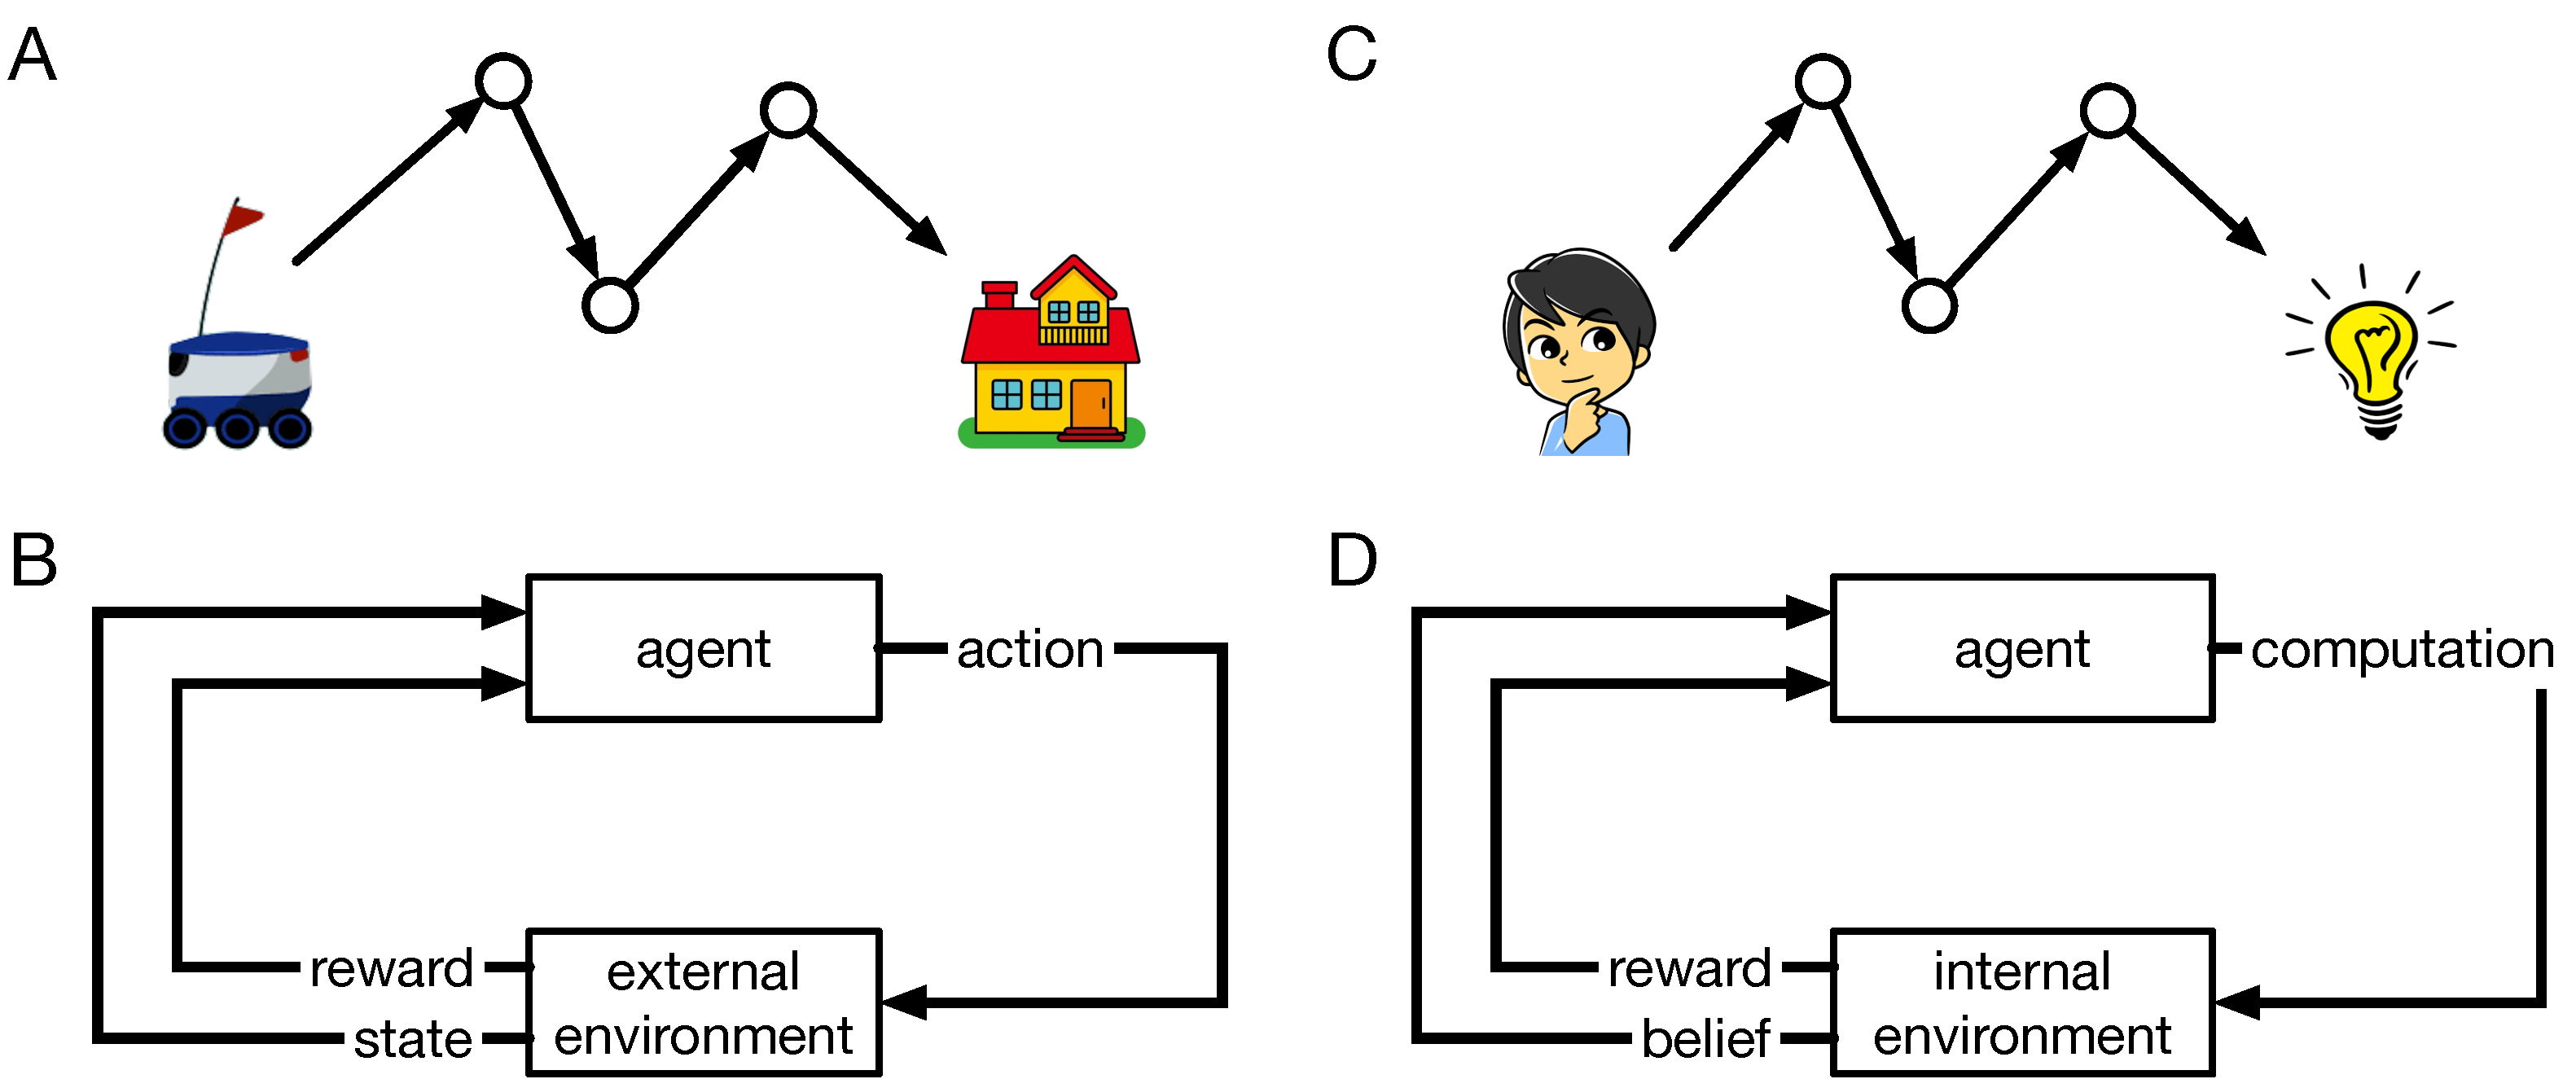
\includegraphics[width=0.9\textwidth]{diagrams/sequential-intuition.pdf}
  \caption{Sequential decision problems posed by external and internal environments.}
  \label{fig:sequential-intuition}
\end{figure}

In the first two chapters,

What does it mean to say that cognition is a sequential decision problem? One way to understand this claim is as an analogy between the type of problems posed by our external, physical environments and the type of problems posed by our internal, mental environments. To make things concrete, consider the problem facing a delivery robot, illustrated in \figref{fig:sequential-intuition}{a}. Completing the delivery will require visiting a sequence of locations before arriving at the final destination. And at each location, the robot will need to decide where to go next. Thus, the robot faces a sequential decision problem. \figref{fig:sequential-intuition}{b} illustrates how this type of problem is often modeled in artificial intelligence research: a \emph{Markov decision process}, or MDP. At each time step, an agent (here, the robot) takes an \emph{action} (e.g., driving forward). This action causes the environment to enter a new \emph{state} (e.g., one where the robot is in a new location). Additionally, the agent receives a \emph{reward}, a number that captures how good or bad the immediate consequences of the action are. For example, the delivery robot might receive a large positive reward for reaching the destination and a small negative reward every time it moves (capturing the desire to conserve battery life). The robot's goal is to maximize the total reward received.
% After receiving the reward and new state, the agent selects another action and the cycle continues.

\figref{fig:sequential-intuition}{c} illustrates a seemingly very different type of situation: a person trying to come up with a solution to a difficult problem. However, as the diagram suggests, the two cases actually share the same basic structure. Both involve an extended interaction between an agent and an environment; but whereas the robot is interacting with an \emph{external} environment, the thinker is interacting with an \emph{internal} environment: their own mind. Just as the robot makes several moves, and visits several locations before reaching the destination, the thinker has several thoughts, and enters several mental states before discovering the solution. Indeed, as illustrated in \figref{fig:sequential-intuition}{d}, this problem can be modeled in precisely the same way as the delivery problem. However, now the actions correspond to \emph{computations} and the states correspond to \emph{mental states}. Thinking changes one's mental state just as moving changes one's physical state; and it also incurs a cost---at the very least, thinking takes time. Because this MDP describes the metacognitive problem of how to interact with one's own mind, it is called a \emph{metalevel} MDP.

The power of identifying this parallel between external and internal environments is that it allows us to leverage existing knowledge about how to solve MDPs (a substantial chunk of AI research) to build rational mechanistic models of cognition. Indeed, this parallel was identified many years ago by researchers in \emph{rational metareasoning}, a subfield of artificial intelligence that aims to construct artificial agents that make effective use of their limited computational resources \citep{russell1991principles,hay2016principles}. My dissertation simply applies the theoretical tools developed there (in particular metalevel MDPS) to a different problem: reverse-engineering an existing intelligent system that makes effective use of its limited resources---the human mind.

\subsection{Attention}

Consider the problems faced by a diner at a buffet table or a shopper at a supermarket shelf. They are presented with a number of options and must evaluate them until they identify the most desirable one. Previous work suggests that these decisions are made by integrating noisy evidence about the value of each alternative, which is sampled over time. Moreover, this process is guided by visual attention, such that the evidence is strongest for the item currently being looked at; as a result, what we look at has consequences for what we choose \citep{krajbich2010visual}. This raise an important question: \textbf{How do we decide what to pay attention to when making
decisions?}

This problem is naturally cast as a metalevel MDP. The (mental) states correspond to the agent's current estimates of (and uncertainty about) the value of each item. The computations correspond to fixating on a given option, drawing a noisy sample of its value, and integrating that information into the corresponding value estimate by Bayesian inference. This sampling and updating process is encoded by the transition function. Finally, the reward function imposes a fixed cost for each sample, an additional switching cost for saccades, and a reward equal to the true value of the chosen option.

Solving this metalevel MDP reveals that it is optimal to attend to options whose value estimates are both uncertain and high---although the latter only holds when choosing between more than two items. We compare these predictions to existing datasets in which participants selected between two or three junk food items while under eye tracking. Consistent with the model's predictions, we find that people balance fixation time to each item in order to keep the uncertainty of each item at similar levels, and---in the case of trinary, but not binary choice---they preferentially attend to items that they rated highly in an earlier phase of the experiment. Furthermore, this effect becomes stronger over time, consistent with the model's assumption that fixations are driven by the evolving belief state.

This chapter is based on a paper which was published in \emph{PLoS Computational Biology} \citep{callaway2021fixation}.

\subsection{Memory}

Consider next the all-too-familiar situation of running into someone whose name you cannot recall. If it feels as though the name is about to come to you, you may pause before saying hello. But every moment you delay only exacerbates the awkwardness of the situation. \textbf{How do people know when to give up on searching for a memory?}

Most empirical work on metacognition in the domain of memory (or ``metamemory'') has focused on how people are able to monitor their memory states \citep{reder1992determines,miner1994new,eakin2005illusions,hart1965memory,vesonder1985ability,dunlosky1992importance,dunlosky2007metacomprehension}. Less emphasis, however, has been placed on understanding the function of metamemory judgments \citep{schwartz2017metamemory}. Although an influential verbal theory suggests that these judgements support metacognitive control of memory through an iterative process of search and re-evaluation \citep{nelson1990metamemory}, this theory has not yet been formalized computationally, making it challenging to rigorously evaluate the theory.

In this chapter, I provide such a formalization, modeling the decision of when to terminate a memory search as a metalevel MDP. Here, the mental states define how close one is to recalling a target memory, and the computations correspond to continuing to search for the target. The transition function describes how recall progress noisly accumulates through search; finnaly,the reward function encodes the value of recalling the item (when a threshold level of progress is reached) and a fixed cost for each moment spent searching.

Solving this metalevel MDP reveals that, unsurprisingly, it is optimal to give up more quickly on a weak memory that for which recall progresses slowly. The model thus captures a consistent empirical finding that people search longer before giving up on memories that they report having a higher``feeling of knowing'' for \citealp{nelson1984comparison,nhouyvanisvong1998rapid,gruneberg1977methodological,lachman1979metamemory}.

One weakness with the above finding, and indeed with many empirical results in metamemory, is that we observe at most one single metacognitive decision in each trial, the decision to terminate search. To provide a stronger test of the sequential search-evaluate loop, my colleagues and I designed a modified cued-recall paradigm in which two candidate memories could be recalled on each trial. By tracking attention to the corresponding cues using a keypress-contingent display, we could observe this metacognitive process unfolding even before a memory was recalled or given up on. Interestingly, contrary to the decision-making case studied in the previous chapter, we see that the optimal policy preferentially attends to cues associated with stronger memories even when there are only two options. Participants showed the same pattern.

This chapter is based on a preprint that is currently under review at \emph{Psychological Review}.

\subsection{Planning}

Finally, consider the problem faced by a traveler in an unfamiliar country, deciding which cities to visit. Geographical concerns limit which cities he can travel between, so his first stop will shape the whole trip. But there are far too many possible routes to consider every one. \textbf{How do we know which hypothetical courses of action to evaluate?}

How people solve problems that require thinking multiple steps ahead has been a focal question since the very earliest attempts to understand the human mind in computational terms \citep{newell1956logic,newell1972human}. Both then and now, most work on human planning has focused on identifying the heuristics people use to select which possibile actions to consider \citep{huys2015interplay}. However, the questions of why people use those particular heuristics and of predicting which of the many possible heuristics people will employ in any particular case, have been relatively unexplored.

To provide a normative theory of human planning strategies and how they adapt to the structure of the environment, we can model planning---specifically, decision tree search---as a metalevel MDP. The mental states correspond to partially constructed decision tree, which represent possible sequences of actions and outcomes. The computations correspond to ``node expansion'', considering a possible future state and expanding the decision tree. TRANSTION AND REWARD.

% To address these questions, we model planning as a metalevel MDP in which states correspond to partially constructed plans (in technical terms, decision trees) and actions correspond to considering possible modifications of those plans (expanding nodes in the decision tree). 

% Solving this metalevel MDP yields an optimal planning algorithm. This algorithm demonstrates many of the previously proposed heuristics, but also some novel ones. Comparing these predictions to human behavior in a process tracing paradigm that externalizes planning operations as information-gathering clicks, we find that people use these heuristics as well. However, when they use each heuristic depends on the structure of the environment, in exactly the way the model predicts.

This work has been written up as a preprint \citep{callaway2021human}. We are about to submit to \emph{Nature Human Behavior}.


\subsection{Conclusion}

Across all three domains, my dissertation research shows how Simon's 1955 insight---that cognitive processes are shaped by the environments both within and outside the mind---can be formalized to generate rational mechanistic models that explain both how and why cognitive processes are the way they are.

\pagebreak

\renewenvironment{APACrefURL}[1][]{}{}
\renewcommand{\url}[1]{}
\renewenvironment{APACrefDOI}[1][]{}{}
\renewcommand{\doi}[1]{}

\bibliography{references}


\end{document}